\documentclass[tikz,border=7pt]{standalone}
\usepackage{tikz}
\usetikzlibrary{arrows.meta,backgrounds,fit,positioning}

\tikzset{
  input/.style={draw, rounded corners=2pt, fill=black!6, align=center,
    text width=29mm, minimum height=9mm, font=\small},
  process/.style={draw, rounded corners=2pt, fill=black!2, align=center,
    text width=30mm, minimum height=10mm, font=\small},
  output/.style={draw, rounded corners=2pt, fill=black!13, align=center,
    text width=31mm, minimum height=10mm, font=\small},
  group/.style={draw, dashed, rounded corners=2pt, inner sep=5mm},
  flow/.style={-{Latex[length=2.1mm]}, line width=.55pt},
  aux/.style={-{Latex[length=1.8mm]}, dashed, line width=.45pt},
  label/.style={font=\scriptsize, fill=white, inner sep=1.2pt},
}

\begin{document}
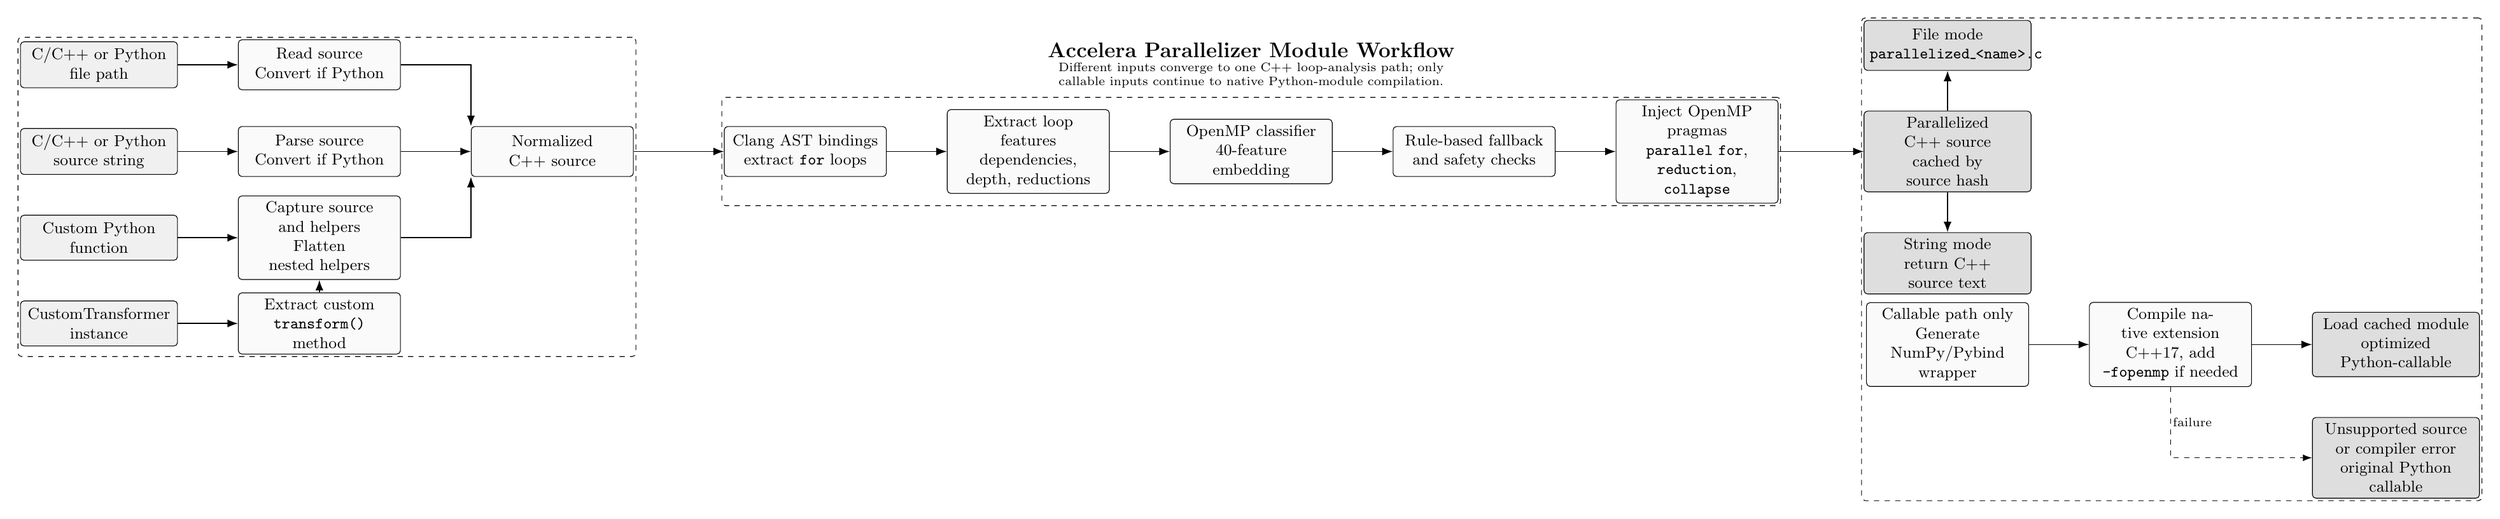
\begin{tikzpicture}[node distance=8mm and 12mm]

% Input normalization panel
\node[input] (file) {C/C++ or Python\\file path};
\node[input, below=8mm of file] (string) {C/C++ or Python\\source string};
\node[input, below=8mm of string] (function) {Custom Python\\function};
\node[input, below=8mm of function] (transformer) {CustomTransformer\\instance};

\node[process, right=of file] (filecode) {Read source\\Convert if Python};
\node[process, right=of string] (stringcode) {Parse source\\Convert if Python};
\node[process, right=of function] (functioncode) {Capture source and helpers\\Flatten nested helpers};
\node[process, right=of transformer] (methodcode) {Extract custom\\\texttt{transform()} method};

\node[process, right=14mm of stringcode] (cppsource) {Normalized C++ source};

\draw[flow] (file) -- (filecode);
\draw[flow] (string) -- (stringcode);
\draw[flow] (function) -- (functioncode);
\draw[flow] (transformer) -- (methodcode);
\draw[flow] (filecode.east) -| (cppsource.north west);
\draw[flow] (stringcode) -- (cppsource);
\draw[flow] (functioncode.east) -| (cppsource.south west);
\draw[flow] (methodcode.north) -- (functioncode.south);

\begin{scope}[on background layer]
\node[group, fit=(file)(transformer)(filecode)(methodcode)(cppsource),
  label={[font=\small\bfseries, fill=white]above:1.5mm:Input normalization}] {};
\end{scope}

% Shared analysis panel
\node[process, right=18mm of cppsource] (ast) {Clang AST bindings\\extract \texttt{for} loops};
\node[process, right=of ast] (features) {Extract loop features\\dependencies, depth, reductions};
\node[process, right=of features] (classifier) {OpenMP classifier\\40-feature embedding};
\node[process, right=of classifier] (rules) {Rule-based fallback\\and safety checks};
\node[process, right=of rules] (pragma) {Inject OpenMP pragmas\\\texttt{parallel for}, \texttt{reduction}, \texttt{collapse}};

\draw[flow] (cppsource) -- (ast);
\draw[flow] (ast) -- (features);
\draw[flow] (features) -- (classifier);
\draw[flow] (classifier) -- (rules);
\draw[flow] (rules) -- (pragma);

\begin{scope}[on background layer]
\node[group, fit=(ast)(pragma),
  label={[font=\small\bfseries, fill=white]above:1.5mm:Shared loop analysis and pragma selection}] {};
\end{scope}

% Output panel
\node[output, right=17mm of pragma] (parallelcode) {Parallelized C++ source\\cached by source hash};
\node[output, above=8mm of parallelcode] (fileout) {File mode\\\texttt{parallelized\_<name>.c}};
\node[output, below=8mm of parallelcode] (stringout) {String mode\\return C++ source text};
\draw[flow] (pragma) -- (parallelcode);
\draw[flow] (parallelcode) -- (fileout);
\draw[flow] (parallelcode) -- (stringout);

\node[process, below=22mm of parallelcode] (wrapper) {Callable path only\\Generate NumPy/Pybind wrapper};
\node[process, right=of wrapper] (compile) {Compile native extension\\C++17, add \texttt{-fopenmp} if needed};
\node[output, right=of compile] (native) {Load cached module\\optimized Python-callable};
\node[output, below=8mm of native] (fallback) {Unsupported source or compiler error\\original Python callable};

\draw[flow] (wrapper) -- (compile);
\draw[flow] (compile) -- (native);
\draw[aux] (compile.south) |- node[label, near start, right] {failure} (fallback.west);

\begin{scope}[on background layer]
\node[group, fit=(parallelcode)(fileout)(stringout)(wrapper)(native)(fallback),
  label={[font=\small\bfseries, fill=white]above:1.5mm:Output modes, caching, and safe fallback}] {};
\end{scope}

\node[above=11mm of classifier, font=\large\bfseries] {Accelera Parallelizer Module Workflow};
\node[above=5mm of classifier, font=\scriptsize, text width=88mm, align=center] {Different inputs converge to one C++ loop-analysis path; only callable inputs continue to native Python-module compilation.};

\end{tikzpicture}
\end{document}
